\documentclass{../../../oss-apphys}

\begin{document}
\genheader

\gentitle{1}{CIRCULAR MOTION AND GRAVITY}

\genmultidirections

\gengravity

\raggedcolumns
\begin{multicols}{2}

  \begin{enumerate}[leftmargin=18pt]  
  \item Two satellites of equal mass orbit a planet. Satellite B orbits at twice
    the orbital radius of Satellite A. Which of the following statements is
    true?
    \begin{enumerate}[nosep,leftmargin=18pt,label=(\Alph*)]
    \item The gravitational force on Satellite A is four times less than that on
      Satellite B.
    \item The gravitational force on Satellite A is two times less than that on
      Satellite B.
    \item The gravitational force on the satellites is equal.
    \item The gravitational force on Satellite A is two times greater than that
      on Satellite B.
    \item The gravitational force on Satellite A is four times greater than that
      on Satellite B.
    \end{enumerate}
    \vspace{.8in}
    
  \item A \SI{70}{\kilo\gram} astronaut floats at a distance of \SI{10}{\metre}
    from a \SI{50000}{\kilo\gram} spacecraft. What is the force of attraction
    between the astronaut and spacecraft?
    \begin{enumerate}[nosep,leftmargin=18pt,label=(\Alph*)]
    \item\SI{2.4e-6}{\newton}
    \item\SI{2.4e-5}{\newton}
    \item Zero; there is no gravity in space.
    \item\SI{2.4e5}{\newton}
    \item\SI{2.4e6}{\newton}
    \end{enumerate}
    \vspace{.8in}
    
  \item The centripetal acceleration on \SI{1000}{\kilo\gram} car in a turn is
    \SI{1e5}{m/s^2}. The radius of the turn is \SI{10}{\metre}. What is the
    car's speed?
    \begin{enumerate}[nosep,leftmargin=18pt,label=(\Alph*)]
    \item\SI{1e1}{\metre\per\second}
    \item\SI{1e2}{\metre\per\second}
    \item\SI{1e3}{\metre\per\second}
    \item\SI{1e4}{\metre\per\second}
    \item\SI{1e5}{\metre\per\second}
    \end{enumerate}
    \columnbreak
    
  \item A proposed ``space elevator'' can lift a \SI{1000}{\kilo\gram} payload
    to an orbit of \SI{150}{\kilo\metre} above the Earth's surface. The radius
    of the Earth is \SI{6.4e6}{\metre}, and the Earth's mass is
    \SI{6.e24}{\kilo\gram}. What is the gravitational potential energy of the
    payload when it reaches orbit?
    \begin{enumerate}[nosep,leftmargin=18pt,label=(\Alph*)]
    \item\SI{1.0e3}{\joule}
    \item\SI{2.7e6}{\joule}
    \item\SI{6.1e10}{\joule}
    \item\SI{2.7e12}{\joule}
    \item\SI{1.0e15}{\joule}
    \end{enumerate}

  \item A satellite orbits the Earth at a distance of \SI{200}{\km}. If the mass
    of the Earth is \SI{6.e24}{\kilo\gram} and the Earth's radius is
    \SI{6.4e6}{\metre}, what is the satellite's speed?
    \begin{enumerate}[nosep,leftmargin=18pt,label=(\Alph*)]
    \item\SI{1.e3}{\metre\per\second}
    \item\SI{3.5e3}{\metre\per\second}
    \item\SI{7.8e3}{\metre\per\second}
    \item\SI{5e6}{\metre\per\second}
    \item\SI{6.1e7}{\metre\per\second}
    \end{enumerate}

  \item Mars orbits the Sun at a distance of \SI{2.3e11}{\metre}. The mass of
    the Sun is \SI{2.e30}{\kilo\gram}, and the mass of Mars is
    \SI{6.4e23}{\kilo\gram}. Approximately what is the gravitational force that
    the Sun exerts on Mars?
    \begin{enumerate}[nosep,leftmargin=18pt,label=(\Alph*)]
    \item\SI{1.6e20}{\newton}
    \item\SI{1.6e21}{\newton}
    \item\SI{3.7e21}{\newton}
    \item\SI{3.7e32}{\newton}
    \item\SI{3.7e42}{\newton}
    \end{enumerate}
    \columnbreak
    
  \item When climbing from sea level to the top of Mount Everest, a hiker
    changes elevation by \SI{8848}{\metre}. By what percentage will the
    gravitational field of the Earth change during the climb? (The Earth's
    mass is \SI{6.e24}{\kilo\gram}, and its radius is \SI{6.4e6}{\metre}.)
    \begin{enumerate}[nosep,leftmargin=18pt,label=(\Alph*)]
    \item It will increase by approximately \SI{.3}{\percent}.
    \item It will decrease by approximately \SI{.3}{\percent}.
    \item It will increase by approximately \SI{12}{\percent}.
    \item It will decrease by approximately \SI{12}{\percent}.
    \item The gravitational field strength will not change.
    \end{enumerate}
    \vspace{.8in}
    
  \item Four planets, A through D, orbit the same star. The relative masses and
    distances from the star for each planet are shown in the table. For
    example, Planet A has twice the mass of Planet B, and Planet D has
    three times the orbital radius of Planet A. Which planet has the highest
    gravitational attraction to the star?
    \begin{center}
      \vspace{-.1in}
      \begin{tabular}{lll}
        \hline
        \textbf{Planet} & \textbf{Relative mass} & \textbf{Relative distance}\\
        \hline
        A\hspace{.4in}& $2m$     & $r$    \\ \hline
        B & $m$                  & $0.1r$\hspace{.25in} \\ \hline
        C & $0.5m$\hspace{.25in} & $2r$   \\ \hline
        D & $4m$                 & $3r$   \\ \hline
      \end{tabular}
    \end{center}
    \begin{enumerate}[nosep,leftmargin=18pt,label=(\Alph*)]
    \item Planet A
    \item Planet B
    \item Planet C
    \item Planet D
    \item All have the same gravitational attraction to the star.
    \end{enumerate}
    \vspace{.8in}
    
  \item A satellite orbits the Earth at a distance that is four times the radius
    of the Earth. If the acceleration due to gravity near the surface of the
    Earth is $g$, the acceleration of the satellite is most nearly
    \begin{enumerate}[nosep,leftmargin=18pt,label=(\Alph*)]
    \item zero
    \item $g/2$
    \item $g/4$
    \item $g/8$
    \item $g/16$
    \end{enumerate}

  \item The mass of a planet is $1/4$ that of Earth and its radius is half of
    Earth's radius. The acceleration due to gravity on this planet is most
    nearly
    \begin{enumerate}[nosep,leftmargin=18pt,label=(\Alph*)]
    \item\SI{2}{\metre\per\second\squared}
    \item\SI{4}{\metre\per\second\squared}
    \item\SI{5}{\metre\per\second\squared}
    \item\SI{10}{\metre\per\second\squared}
    \item\SI{20}{\metre\per\second\squared}
    \end{enumerate}
  
%  \item A satellite orbits the Earth in an elliptical orbit, with point A being
%    close to the Earth and point B farther away. As the satellite moves from
%    point A to point B, which of the following is true of the angular momentum
%    and kinetic energy of the satellite?
%    \begin{center}
%      \vspace{-.1in}
%      \begin{tikzpicture}[scale=1.4]
%        \tikzstyle{balloon}=[ball color=gray];
%        \draw(0,0) ellipse (2 and 1);
%        \draw[fill=black](2,0) circle(0.05) node[right]{A};
%        \draw[fill=black](-2,0) circle(0.05) node[left]{B};
%        \shade[balloon] (0.5,0) circle (0.2);
%      \end{tikzpicture}
%    \end{center}
%  
%    \begin{tabular}{lll}
%      & \underline{Angular momentum} & \underline{Kinetic energy}\\
%      (a) & Increases & Remains constant \\
%      (b) & Remains constant & Increases \\
%      (c) & Decreases & Remains constant \\
%      (d) & Remains constant & Decreases \\
%      (e) & Remains constant & Remains constant
%    \end{tabular}
    
  \item Two planets of mass $M$ and $9M$ are in the same solar system. The
    radius of the planet of mass $M$ is $R$. In order for the acceleration due
    to gravity to be the same for each planet, the radius of the planet of mass
    $9M$ would have to be
    \begin{enumerate}[nosep,leftmargin=18pt,label=(\Alph*)]
    \item $R/2$
    \item $R$
    \item $2R$
    \item $3R$
    \item $9R$
    \end{enumerate}
    %\vspace{-.5in}
    
  \item Two planets, X and Y, orbit a star. Planet X orbits at a radius $R$, and
    Planet Y orbits at a radius $3R$. Which of the following best represents
    the relationship between the acceleration $a_X$ of Planet X and the
    acceleration $a_Y$ of Planet Y?
    \begin{center}
      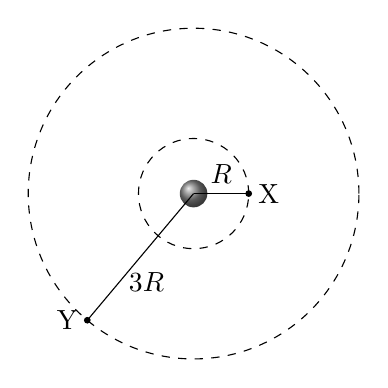
\begin{tikzpicture}[scale=.7]
        \tikzstyle{balloon}=[ball color=gray];
        \shade[balloon](0,0) circle(.25);
        \draw[dashed](0,0) circle(1);
        \draw[dashed](0,0) circle(3);
        \draw(0,0)--(1,0) node[pos=1,right]{X} node[midway,above]{$R$};
        \draw[fill=black](1,0) circle(.05);
        \begin{scope}[rotate=230]
          \draw(0,0)--(3,0) node[pos=1,left]{Y} node[pos=0.7,right]{$3R$};
          \draw[fill=black](3,0) circle(.05);
        \end{scope}
      \end{tikzpicture}
    \end{center}
    \begin{enumerate}[nosep,leftmargin=18pt,label=(\Alph*)]
    \item $a_X = 9a_Y$
    \item $9a_X = a_Y$
    \item $a_X = 3a_Y$
    \item $3a_X = a_Y$
    \item $a_X = a_Y$
    \end{enumerate}
  \item A satellite is in a stable circular orbit around the Earth at a radius
    $R$ and speed $v$. At what radius would the satellite travel in a stable
    orbit with a speed $2v$?
    \begin{enumerate}[nosep,leftmargin=18pt,label=(\Alph*)]
    \item $1⁄4\;R$
    \item $1⁄2\;R$
    \item $R$
    \item $2R$
    \item $4R$
    \end{enumerate}

    \columnbreak

  \item The Earth and the moon apply a gravitational force to each other.
    Which of the following statements is true?
    \begin{enumerate}[nosep,leftmargin=18pt,label=(\Alph*)]
    \item The Earth applies a greater force on the moon than the moon exerts on
      the Earth.
    \item The Earth applies a smaller force on the moon than the moon exerts on
      the Earth.
    \item The Earth applies a force on the moon, but the moon does not exert a
      force on the Earth.
    \item The Earth does not apply a force on the moon, but the moon exerts a
      force on the Earth.
    \item The force the Earth applies to the moon is equal and opposite to the
      force the moon applies to the Earth.
    \end{enumerate}
    \vspace{.8in}
  \item Two masses exert a gravitational force $F$ on each other. If one of the
    masses is doubled, and the distance between the masses is tripled, the
    new force between them is
    \begin{enumerate}[nosep,leftmargin=18pt,label=(\Alph*)]
    \item $6F$
    \item $2F/3$
    \item $2F/9$
    \item $3F/2$
    \item $4F/9$
    \end{enumerate}

  \item A planet orbits at a radius $R$ around a star of mass $M$. The period of
    orbit of the planet is
    \begin{enumerate}[nosep,leftmargin=18pt,label=(\Alph*)]
    \item $\displaystyle\sqrt{\frac{4\pi^2R^2}{GM}}$
    \item $\displaystyle\frac{4\pi^2R^3}{GM}$
    \item $\displaystyle\sqrt{\frac{4\pi^2R^3}{GM}}$
    \item $\displaystyle\sqrt{\frac{4\pi^2R}{GM}}$
    \item $\displaystyle\frac{GM}{4\pi^2R}$
    \end{enumerate}
    \columnbreak

%  \item A moon orbits a large planet in an elliptical orbit, with its closest
%    approach at a distance $a$, and its farthest distance $b$. The speed of the
%    moon at point b is $v$. The speed at point $a$ is
%    \begin{enumerate}[nosep,leftmargin=18pt,label=(\Alph*)]
%    \item $\displaystyle\frac{av}{b}$
%    \item $\displaystyle\frac{bv}{a}$
%    \item $\displaystyle\frac{(a+b)v}{b}$
%    \item $\displaystyle\frac{(b-a)v}{b}$
%    \item $\displaystyle\frac{2bv}{a}$
%    \end{enumerate}

%  \item A satellite orbits the Earth in an elliptical orbit. Which of the
%    following statements is true?
%    \begin{enumerate}[nosep,leftmargin=18pt,label=(\Alph*)]
%    \item The angular velocity of the satellite increases as it travels farther
%      from the Earth.
%    \item The acceleration of the satellite increases as it travels closer to
%      the Earth.
%    \item The angular momentum of the satellite increases as it travels closer
%      to the Earth.
%    \item The potential energy of the satellite is equal to its kinetic energy
%      at all points in the orbit.
%    \item The speed of the satellite must remain constant for it to remain
%      in orbit around the Earth.
%    \end{enumerate}
%
%  \item Two moons of mass $m$ and $2m$ orbit a planet of mass $M$ at the same
%    radius $R$ and speed $v$ toward each other, as shown. The moons collide and
%    stick together without destroying either moon. The total momentum of the
%    moons after the collision is
%    \begin{center}
%      \begin{tikzpicture}[scale=0.8]
%        \tikzstyle{balloon}=[ball color=gray];
%        \shade[balloon] circle(.25) node[below]{$M$};
%        \draw[dashed](0,0) circle(3);
%        \begin{scope}[rotate=50]
%          \draw[->](0.25,0)--(2.8,0) node[midway,right]{$R$};
%          \shade[balloon] (3,0) circle (0.2) node[right]{$m$};
%          \draw[thick,->](3,0.25)--(3,1.25) node[pos=1,above]{$v$};
%        \end{scope}
%        \begin{scope}[rotate=130]
%          \shade[balloon] (3,0) circle (0.2) node[left]{$2m$};
%          \draw[thick,->](3,-0.25)--(3,-1.25) node[pos=1,above]{$v$};
%        \end{scope}
%      \end{tikzpicture}
%    \end{center}
%    \begin{enumerate}[nosep,leftmargin=18pt,label=(\Alph*)]
%    \item $mv$
%    \item $2mv$
%    \item $3mv$
%    \item $6mv$
%    \item zero
%    \end{enumerate}
%
%    \columnbreak
%    
%  \item The velocity of the two masses after the collision above is
%    \begin{enumerate}[nosep,leftmargin=18pt,label=(\Alph*)]
%    \item $v$ counterclockwise
%    \item $v/2$ counterclockwise
%    \item $v/2$ clockwise
%    \item $v/3$ counterclockwise
%    \item $v/3$ clockwise
%    \end{enumerate}

  \item Consider a two-star system shown above, which consists of two stars of
    mass $m$ rotating in a circle of radius $r$ about their center of mass. What
    is the total energy of the two-star system?
    \begin{enumerate}[nosep,leftmargin=18pt,label=(\Alph*)]
    \item $-Gm^2/2r$
    \item $Gm^2/2r$
    \item $Gm^2/4r$
    \item $3Gm^2/4r$
    \item $-Gm^2/4r$
    \end{enumerate}

  \item If a planet has twice the radius of Earth and half of Earth's density,
    what is the acceleration due to gravity on the surface of the planet (in
    terms of the gravitational acceleration $g$ on the surface of Earth)?
    \begin{enumerate}[nosep,leftmargin=18pt,label=(\Alph*)]
    \item $4g$
    \item $2g$
    \item $g$
    \item $g/2$
    \item $g/4$
    \end{enumerate}
  \end{enumerate}
\end{multicols}

\newpage
\genfreetitle{1}{CIRCULAR MOTION AND GRAVITY}{5}

\genfreedirections

% THIS QUESTION IS FROM THE 2001 AP PHYSICS B FREE RESPONSE QUESTION #1
\begin{center}
  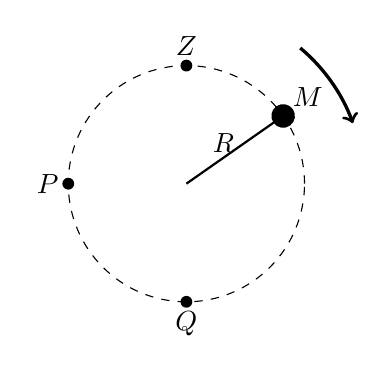
\begin{tikzpicture}[scale=.5]
    \draw[dashed](0,0) circle(3);
    \fill(-3,0) circle(.15) node[left]{$P$};
    \fill(0,-3) circle(.15) node[below]{$Q$};
    \fill(0,3) circle(.15) node[above]{$Z$};
    \draw[very thick,rotate=50,->](4.5,0) arc(0:-30:4.5);
    \begin{scope}[rotate=35]
      \draw[thick](0,0)--(3,0) node[pos=.6,left]{$R$};
      \fill(3,0) circle(.3) node[above right]{$M$};
    \end{scope}
  \end{tikzpicture}
\end{center}
\begin{enumerate}[leftmargin=15pt]
\item A ball of mass $M$ is attached to a string of length $R$ and negligible
  mass. The ball moves clockwise in a vertical circle, as shown above. When the
  ball is at point $P$, the string is horizontal. Point $Q$ is at the bottom of
  the circle and point $Z$ is at the top of the circle. Air resistance is
  negligible. Express all algebraic answers in terms of the given quantities
  and fundamental constants.
  \begin{enumerate}[noitemsep]
  \item On the figures below, draw and label all the forces exerted on the ball
    when it is at points $P$ and $Q$, respectively.
    \begin{center}
      \begin{tikzpicture}[scale=.4]
        \draw[dashed](0,0) circle(3);
        \fill(-3,0) circle(.25) node[left]{$P$};
        \draw[very thick,rotate=-75,->](3.5,0) arc(0:-30:3.5);
      \end{tikzpicture}
      \hspace{1in}
      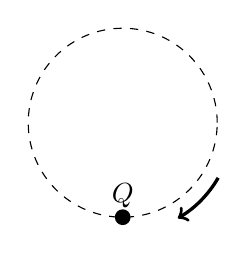
\begin{tikzpicture}[scale=.4]
        \draw[dashed](0,0) circle(3);
        \fill(0,-3) circle(.25) node[above]{$Q$};
        \draw[very thick,rotate=-30,->](3.5,0) arc(0:-30:3.5);
      \end{tikzpicture}
    \end{center}
    \vspace{.3in}
  \item Derive an expression for $v_\mathrm{min}$, the minimum speed the ball
    can have at point $Z$ without leaving the circular path.
  \item The maximum tension the string can have without breaking is
    $T_\mathrm{max}$. Derive an expression for $v_\mathrm{min}$, the maximum
    speed the ball can have at point $Q$ without breaking the string.
  \item Suppose that the string breaks at the instant the ball is at point $P$.
    Describe the motion of the ball immediately after the string breaks.
  \end{enumerate}
  \newpage
  
%\item Two meteoroids are \SI{250000}{\kilo\metre} from Earth's center and moving
%  at \SI{2.1}{\kilo\metre\per\second}. One is headed straight for Earth, while
%  the other is on a path that will come within \SI{8500}{\kilo\metre} of Earth's
%  center. Find the speed of
%  \begin{enumerate}[noitemsep,leftmargin=20pt]
%  \item the first meteoroid when it strikes Earth, and
%  \item the second meteoroid at its closest approach.
%  \item Will the second meteoroid ever return to Earth's vicinity?
%  \end{enumerate}
%  \vspace{2.5in}

\item Two stars of equal mass $M$ are orbiting each other in a circular path.
  Show that the orbital period is given by:
  \begin{displaymath}
    T^2=\frac{2\pi^2d^3}{GM}
  \end{displaymath}
  where $d$ is the distance between the stars.
  \vspace{\stretch{1}}
  
%\item A planet of mass $M$, radius $R$, and uniform density has a small tunnel
%  drilled through the center of the planet, as shown below. When the mass is
%  inside the tunnel, it experiences a force of $F=(GmM/R^3)r$, whereas when the
%  mass is outside of the planet, it experiences a gravitational force of
%  $F=GmM/r^2$.
%  \begin{center}
%    \begin{tikzpicture}
%      \draw(0,0) circle(2);
%      \draw(-0.1,2) rectangle(0.1,-2);
%      \draw[->,thick,rotate=35](0,0)--(2,0) node[midway,below]{$R$};
%    \end{tikzpicture}
%  \end{center}
%  \begin{enumerate}[noitemsep,leftmargin=20pt]
%  \item Setting the potential energy of the mass to be zero at the planet's
%    center, calculate the mass's potential energy as a function of distance from
%    the center of the planet $U(r)$, for values $r<R$. Sketch this potential
%    function.
%  \item If the mass is dropped from $R$ from the center of the planet, how long
%    will it take until it returns to its original position?
%  \item If the mass is dropped from $R/2$ from the center of the planet, will
%    it require more, or less, or the same amount of time to return to its
%    original position compared to if it was dropped from $R$?
%  \item If the mass is dropped from $2R$ from the center of the planet, will
%    it require more, or less, or the same amount of time to return to its
%    original position compared to if it was dropped from $R$?
%  \end{enumerate}
%  \newpage

\item Two stars of unequal mass orbit each other about their common center of
  mass as shown. The star of mass $M_1$ orbits in a circle of radius $r$, and
  the star of mass $M_2$ orbits in a circle of radius $2r$.
  \begin{center}
    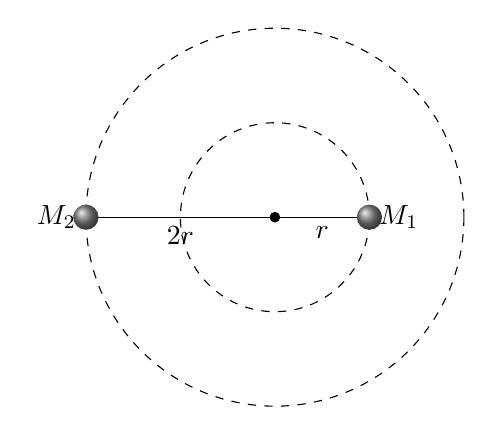
\begin{tikzpicture}[scale=0.8]
      \tikzstyle{balloon}=[ball color=gray];
      \draw[fill=black](0,0) circle(0.075);
      \draw[dashed](0,0) circle(3);
      \draw[dashed](0,0) circle(1.5);
      \draw[->](0,0)--(1.5,0) node[midway,below]{$r$};
      \shade[balloon] (1.5,0) circle (0.2) node[right]{$M_1$};
      \draw[->](0,0)--(-3,0) node[midway,below]{$2r$};
      \shade[balloon] (-3,0) circle (0.2) node[left]{$M_2$};
    \end{tikzpicture}
  \end{center}
  \begin{enumerate}[noitemsep,leftmargin=20pt]
  \item Determine the ratio of masses $M_1/M_2$.
  \item Determine the ratio of the acceleration $a_1$ of $M_1$ to the
    acceleration $a_2$ of $M_2$.
  \item Determine the ratio of the period $T_1$ of $M _1$ to the period $T_2$
    of $M_2$.
  \end{enumerate}
  \vspace{\stretch{1}}
  
%\item As a member of the 2240 Olympic Committee, you are considering a new
%  sport: asteroid jumping. On Earth, world-class high jumpers routinely clear
%  \SI{2}{\metre}. Your job is to make sure athletes jumping from asteroids will
%  return to the asteroid. Make the simplifying assumption that asteroids are
%  spherical, with an average density of \SI{2500}{\kilo\gram\per\metre^3}. For
%  safety, make sure that even a jumper capable of \SI{3}{\metre} on Earth will
%  return to the surface. What do you report for the minimum asteroid diameter?
  \newpage

\item Two point particles of mass $m$ are on the $y$ axis at $y=a$ and $y=-a$,
  as shown in the figure below.
  \begin{center}
    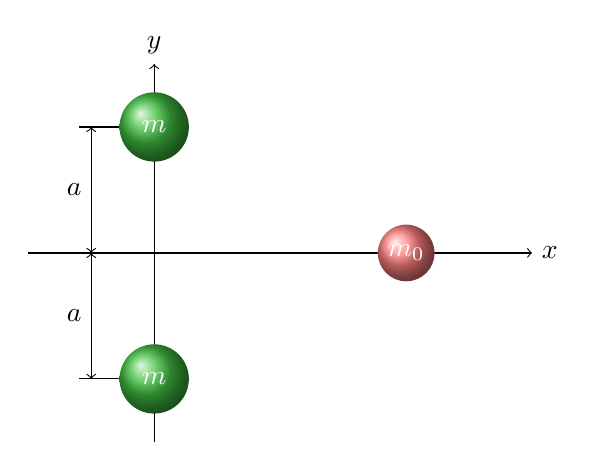
\begin{tikzpicture}[scale=.8]
      \tikzstyle{balloon1}=[ball color=green!50!gray];
      \tikzstyle{balloon2}=[ball color=red!50];
      \draw[->](-2,0)--(6,0) node[pos=1,right]{$x$};
      \draw[->](0,-3)--(0,3) node[pos=1,above]{$y$};
      \draw[<->](-1,0)--(-1,2) node[midway,left]{$a$};
      \draw[<->](-1,0)--(-1,-2)node[midway,left]{$a$};
      \draw(0,2)--(-1.2,2);
      \draw(0,-2)--(-1.2,-2);
      \shade[balloon1] (0,2) circle (.55) node[white]{$m$};
      \shade[balloon1] (0,-2)circle (.55) node[white]{$m$};
      \shade[balloon2] (4,0) circle (.45) node[white]{$m_0$};
    \end{tikzpicture}
  \end{center}
  \begin{enumerate}[noitemsep,leftmargin=20pt]
  \item Derive the expression for the gravitational force exerted by these two
    particles on a third particle of mass $m_0$ located on teh $x$ axis at a
    distance $x$ away from the origin.
  \item What is the gravitational field $\mb{g}$ on the $x$-axis due to the
    two particles?
  \item Show that $g_x$ (the $x$ component of $\mb{g}$) due to the two
    particles on the $y$ axis is approximately $\displaystyle-\frac{2Gm}{x^2}$
    when $x$ is much greater than $a$.
  \item Show that the maximum value of $|g_x|$ occurs at the point
    $\displaystyle x=\frac{\pm a}{\sqrt{2}}$.
  \end{enumerate}
  \newpage

\item Five equal masses $M$ are equally spaced on the arc of a semicircle of
  radius $R$ as shown in the figure below. A mass $m$ is located at the center
  of curvature of the arc. If $M$ is \SI{3}{\kilo\gram}, $m$ is
  \SI{21}{\kilo\gram}, nad $R$ is \SI{10}{\centi\metre}, what is the force on
  $m$ due to the five masses?
  \begin{center}
    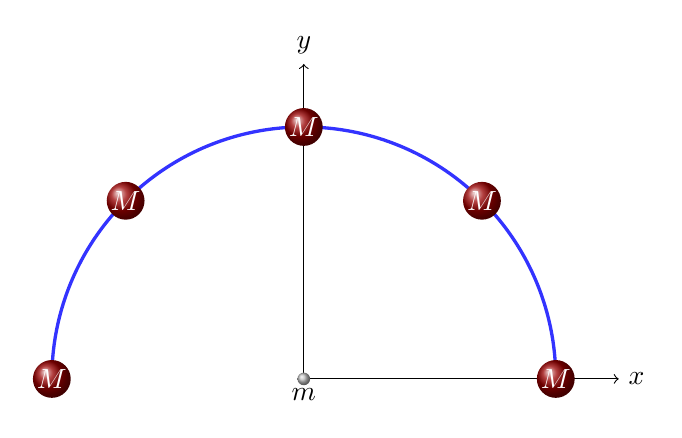
\begin{tikzpicture}[scale=.8]
      \tikzstyle{balloon1}=[ball color=gray!50];
      \tikzstyle{balloon2}=[ball color=red!60!black];
      \draw[->](0,0)--(5,0) node[pos=1,right]{$x$};
      \draw[->](0,0)--(0,5) node[pos=1,above]{$y$};
      \draw[very thick,blue!80](4,0) arc(0:180:4);
      \shade[balloon1] (0,0) circle (.1) node[below]{$m$};
      \foreach \theta in {0,45,...,180} {
        \begin{scope}[rotate=\theta]
          \shade[balloon2] (4,0) circle (.3) node[white]{$M$};
        \end{scope}
      }
    \end{tikzpicture}
  \end{center}
  \vspace{\stretch{1}}
  
%\item\textbf{THIS IS A CHALLENGE PROBLEM THAT IS MORE DIFFICULT THAN AP EXAMS:}
%  Spacecraft that study the Sun are often placed at the ``L1 Lagrange Point'',
%  located sunward of Earth on the Sun--Earth line. L1 is the point where Earth's
%  and Sun's gravity together produce an orbital period of one year, so that a
%  spacecraft at L1 stays fixed relative to Earth as both planet and spacecraft
%  orbit the Sun. This placement ensures an uninterrupted view of the sun,
%  without being periodically eclipsed by Earth as would occur in Earth orbit.
%  Find L1's location relative to Earth. (Hint: This problem calls for numerical
%  methods for solving high-order polynomial equation.)
%  
\end{enumerate}
\end{document}
